\documentclass[lettersize]{sig-alternate-konrad}
\usepackage{listings}
\usepackage{times}  % Use Adobe Times font set
%\usepackage{epsfig,twocolumn}
\usepackage{url}
\usepackage{textcomp}
\usepackage{graphicx} 
\usepackage{color}
\usepackage{multirow}

% This will generate links within the PDF as well as a set of bookmarks
% \usepackage[colorlinks,pdfpagemode=None]{hyperref} 

%% ----- Customizations -----
\setlength{\abovecaptionskip}{-0.05in}
\setlength{\belowcaptionskip}{-0.05in}

\newcommand{\XXXnote}[1]{{\bf\color{red} XXX: #1}}
%\newcommand{\XXXnote}[1]{}

\pagestyle{empty}
%\pagenumbering{arabic}

\begin{document}

%%%%%%%%%%%% THIS IS WHERE WE PUT IN THE TITLE AND AUTHORS %%%%%%%%%%%%

\conferenceinfo{SenSys'08,} {November 5--7, 2008, Raleigh, North Carolina, USA.} 
\CopyrightYear{2008}
\crdata{978-1-59593-990-6/08/11}

\title{{\ttlfnt Lance: Optimizing High-Resolution Signal Collection
in Wireless Sensor Networks}}
\numberofauthors{1}
\author{\alignauthor Geoffrey Werner-Allen$^\dag$, Stephen
Dawnson-Haggerty$^\star$ and Matt Welsh$^\dag$\\
{\affaddr $^\dag$ School of Engineering and
Applied Sciences, Harvard
University, Cambridge, MA 02138} \\
{\affaddr $^\star$ University of California, Berkeley, Berkeley, CA 94720} \\
\email{werner@eecs.harvard.edu, stevedh@cs.berkeley.edu,
mdw@eecs.harvard.edu}
{\affaddr \texttt{http://fiji.eecs.harvard.edu/Lance}}}
\maketitle

\maketitle
\thispagestyle{empty}

%%%%%%%%%%%%%  ABSTRACT GOES HERE %%%%%%%%%%%%%%

\subsection*{Abstract}
An emerging class of sensor networks focuses on reliable 
collection of high-resolution signals from across the network.
In these applications, the system is capable of acquiring more 
data than can be delivered to the base station, 
due to severe limits on radio bandwidth and energy.
Moreover, these systems are unable 
to take advantage of conventional approaches to in-network data
aggregation, given the high data rates and need for raw signals.
These systems face an important challenge: how to
maximize the overall value of the collected data, subject to resource constraints.

In this paper, we describe {\em Lance}, a general approach to
bandwidth and energy management for reliable data collection in wireless
sensor networks. Lance couples the use of optimized, data-driven 
reliable data collection with a model of energy cost for extracting 
data from the network. Lance's design decouples resource allocation 
mechanisms from application-specific policies, enabling flexible 
customization of the system's optimization metrics.

We describe the Lance architecture in detail, demonstrating its
use through a range of target applications and resource management
policies. We present an extensive study driven by both 
real and synthetic data distributions, through simulations and runs
on a large sensor testbed.  We show that Lance maximizes 
the value of the collected data under a range of resource 
constraints, achieving near-optimal allocation of radio bandwidth and
energy. Finally, we present results from a real sensor network
deployment at Tungurahua volcano, Ecuador, in which Lance was used to
drive data collection for an eight-node network collecting seismic and
acoustic signals from the active volcano.  

%%%%%%%%%%%%%  BODY OF PAPER GOES HERE %%%%%%%%%%%%%%


\category{C.2.4}{Distributed Systems}{}
\category{C.3}{Special-Purpose and Application-Based
Systems}{Real-time and embedded systems}
\vspace{-0.1in}
\terms{Design}
\vspace{-0.1in}
\keywords{Wireless Sensor Networks, Data Collection, Resource
Management}

\chapter{Introduction}
\label{chap-intro}

An emerging application for wireless sensor networks is their use in medical
care. Many medical applications place new demands on sensor network designs.
They often involve variable data rates, multiple receivers, and mobile
nodes. Most existing sensor network designs do not adequately support these
requirements, focusing instead on aggregating small amounts of data from nodes
at fixed locations. Therefore a gap exists between existing sensor network
architectures and the requirements of medical applications.

In this dissertation, we bridge the gap by making three contributions: we
propose CodeBlue medical sensor network architecture, TinyADMR ad-hoc multicast routing protocol, and LiveNet passive monitoring infrastructure.
With CodeBlue, we address the challenges of providing a flexible 
and implementable system architecture for mote-based medical
sensor networks. TinyADMR addresses challenges in multicast routing with the
existence of low quality radio links, memory and bandwidth limitations.
LiveNet addresses the challenges for evaluating deployed medical sensor
networks by reconstructing network dynamics without introducing additional
overhead to the network. We evaluate CodeBlue, TinyADMR and LiveNet
with an indoor sensor network testbed and with a disaster drill deployment.

\section{Medical sensor networks}

The convergence of several new hardware technologies, including MEMS, low
power processors, and low power radio, has enabled a new class of computing
platform: wireless sensors. Wireless sensors combine the capability of
sensing, computation, and wireless communication into a single physical
package, enabling a wide range of applications. Over the past decade, sensor
networks research community has explored the use of wireless sensors in
military target tracking and environmental monitoring such as habitats,
forests, volcanoes, civil infrastructures, factory equipments, and home energy
usage.

One common characteristic of most conventional sensor networks is that they
are intended for deployments of stationary nodes that transmit data at
relatively low rates, with a focus on best-effort data collection at a central
base station. Although the sensor networks research community has made
tremendous progress in perfecting networking and operating system support in
this space, we argue that there is a lack of adequate architectural
support for one emerging and important application domain: medical care.

In a hospital or clinic, outfitting every patient with tiny,
wearable wireless vital sign sensors allows doctors, nurses and other
caregivers to continuously monitor the status of their patients.  In
an emergency or disaster scenario, the same technology would enable
medics to more effectively care for large numbers of casualties.
First responders could receive immediate notifications on any changes
in patient status, such as respiratory failure or cardiac arrest.
Wireless sensors can augment or replace existing wired telemetry
systems for many specific clinical applications, such as physical
rehabilitation or long-term ambulatory monitoring.

A typical scenario involves many patients wearing sensors that monitor basic
vital signs such as heart rate or blood oxygen saturation. A small number of
medical personnel are responsible for continuously monitoring the patients
using devices such as laptops or PDAs. Using the real-time information
retrieved from the network, the medical team can treat
patients who need urgent care more efficiently.


\subsection{Application requirements}

Medical sensor networks have several different characteristics than
conventional sensor network applications. The sensors are worn by patients and the
data sinks are mobile computers carried by doctors or nurses so that the nodes
in the network are not stationary. Unlike typical sensor networks, there are
likely to be more than one data sinks in the network. Nodes can also join or
leave the network dynamically. Furthermore, the data traffic pattern is
on-demand and dynamic. Different doctors may be interested in real-time status
of different groups of patients and the groups can potentially overlap. There may
also be interests for different types or resolutions of sensor data.
Conventional sensor network architectures are inadequate in such scenarios
because the system cannot assume fixed sensor queries, sampling rate and
static traffic pattern. 


%% data may have different priorities associated with it

\subsection{Resource limitation}

In addition to meeting a different set of application requirements, medical sensor
networks, as conventional sensor network systems, face the challenges from
severe
resource limitations of the low power sensor platforms. To be practical, the
sensor nodes must be light-weight, low power and low cost so that they can be
wearable, have long enough battery lifetime and be affordable. This entails
the use of low power radio and low power processor.  For example, the mote
platform, MicaZ~\cite{micaz}, that we use for our medical sensor networks has
4~KB of RAM, a 4~MHz 8-bit CPU and a low power IEEE 802.15.4 radio with
maximum transmit power at 0 dBm. The implication of such a limited platform is
that the software running on the mote cannot be overly computationally
intensive or require large amount of memory. Yet, the system must be responsive enough
to handle complex
interactions with the environment such as sampling medical sensors and
performing radio communication in time. As a result, we not only have to find
a new architecture that fulfills the application requirements, it must also be
designed carefully so that it is light weight enough to fit into the platform
but complex enough to fulfill the application demands. 

\section{Systems challenges for medical sensor networks}

We outline a set of challenges identified through the process of designing,
implementing, deploying, and evaluating a medical sensor network. First of
all, there needs to be a new network architecture to efficiently support the
type of queries and traffic patterns for medical sensor networks. Secondly,
to support the new architecture, it is necessary to provide multicast routing
capability on resource-limited sensor nodes. Third, studying a deployed
medical sensor network requires a non-trivial network monitoring infrastructure.

\subsection{A new network architecture}

In contrast to conventional sensor network applications, medical monitoring
must support a large number of patient sensors deployed in a hospital or
disaster site, a variety of data rates, and multiple mobile receiving
devices, such as PDAs carried by doctors or medics. Moreover, medical
monitoring cannot make use of traditional
in-network aggregation since it is not generally meaningful to combine data
from multiple patients. The goal is instead to efficiently deliver information
to the correct receivers. Therefore, there is a significant gap between
existing sensor network designs and the requirements of medical monitoring. 

Supporting such broad range of requirements demands a new approach to
sensor network design. To bridge the technology gap, we propose CodeBlue, an
architecture for medical sensor networks that provides a set of protocols and
services tailored for this application domain. CodeBlue includes
a publish/subscribe communication model, a rich query interface for periodic
and triggered collection of sensor data, a dynamic sensor discovery protocol,
and a programmatic external interface based on Web Services standards.
CodeBlue provides a high-level interface to the network, making it easy to
support new sensor types and applications that tie into real-time medical
sensor data.

\subsection{Multicast on resource limited sensor nodes}

By reviewing the application requirements of medical sensor networks, it
becomes clear that an ad-hoc multicast routing protocol is more adequate
than the conventional many-to-one data collection tree routing approach.
Fortunately there are existing multicast protocols designed for ad-hoc mobile
networks. However, after the attempt to implement one such protocol, ADMR, on
our resource limited sensor platform, we have discovered several challenges
that were not foreseen by the original designers. In order to achieve
acceptable packet delivery ratio, we have to use different routing metrics that
involves the use of link quality information. We have also
investigated the challenges to scale the network within the memory and
bandwidth limitations on the sensor platform.

\subsection{Deployment support}

To find out whether a design is practical for realistic use, one needs to
deploy the network and evaluate the performance in a realistic environment.
For this purpose, we have conducted a deployment study of the CodeBlue
network. It is necessary to record system behavior in order to study
the correctness and performance of the network during the deployment. Under severe
resource constraints on CPU, memory and bandwidth, it is not practical to
record such information on the sensor nodes locally or transmit the logged
information over the radio. To overcome this problem, we have designed and
built LiveNet, an entirely passive monitoring infrastructure for
reconstructing dynamics of deployed sensor networks.  LiveNet is passive and
therefore does not require changing the application code or incur any
additional resource consumption in the network. Yet, it is able provide
valuable information for evaluating and debugging the deployed network.

\section{Dissertation outline}

The remainder of the dissertation is organized as follows.

Chapter 2 considers background and related work. This chapter introduces 
existing work in sensor networks and ad-hoc networking research community that 
are related to medical sensor networks. We also provide an overview of target
hardware platforms of this thesis.

Chapter 3 presents the requirements for a large class of medical sensor
network applications and a new software architecture to meet these
needs. We first propose the CodeBlue network architecture by presenting the
system goals and overall architecture design. We then describe individual
components
to discuss the design trade-offs in detail. Our key contributions include
proposing publish/subscribe as the appropriate networking abstraction for
a medical sensor network and designing CodeBlue Query (CBQ) interface, which
provides a programmatic interface to the medical sensor network.

Chapter 4 presents our approach to achieving efficient publish/subscribe
communication in sensor networks with mobile nodes, based on the
ADMR~\cite{admr-mobihoc01} {\em ad-hoc\/} multicast routing
protocol. We first describe the challenges encountered when designing and 
implementing the multicast layer to support publish/subscribe communication 
model for CodeBlue. We identify the
challenges from unreliable wireless radio links, memory constraints and
bandwidth constraints. We also explore and evaluate different route discovery
and expiration strategies. The key contributions include two new 
routing metrics that exploit link quality information and identifying
scalability limitations from memory and bandwidth constraints.

Chapter 5 describes LiveNet passive monitoring infrastructure. This chapter 
covers the architecture of LiveNet that involves passive sniffers, trace
merging algorithm and a set of analyses that are used to analyze CodeBlue
deployments. We also present the results of an extensive validation study of 
LiveNet's performance and accuracy with a set of controlled experiments with 
an indoor testbed, MoteLab.

Chapter 6 covers implementation and detailed performance evaluation of
CodeBlue network architecture.  We present evaluation of CodeBlue both on a
sensor network testbed and with a disaster drill deployment.  The testbed
experiments evaluate CodeBlue in scalability, fairness, latency, jitter and
effect of mobility. Then we present a deployment study that was part of a disaster
drill simulating a bus accident. Using data from LiveNet, we are able to
analyze the traffic load, network hotspots, routing paths, and query yield for
this deployment.

Chapter 7 contains lessons learned from the experience of 
designing, implementing, deploying and evaluating medical sensor networks and
provide potential future research directions. 

Chapter 8 concludes.

\section{Background}
\label{sec-background}

Networks of spatially-distributed sensors are commonly used to
monitor volcanic activity, both for hazard monitoring and scientific
research~\cite{Scarpa96}.  Typical sensing instruments include
seismic, acoustic, GPS, tilt-meter, optical thermal, and gas
flux. Unfortunately, the number of deployed sensors
at a given volcano has traditionally been limited by a variety of factors,
including monetary expenses such as sensor, communication, and power costs;
logistical concerns related to time and access issues; and archival and
telemetry bandwidth constraints.

\begin{figure*}[t]
\begin{center}
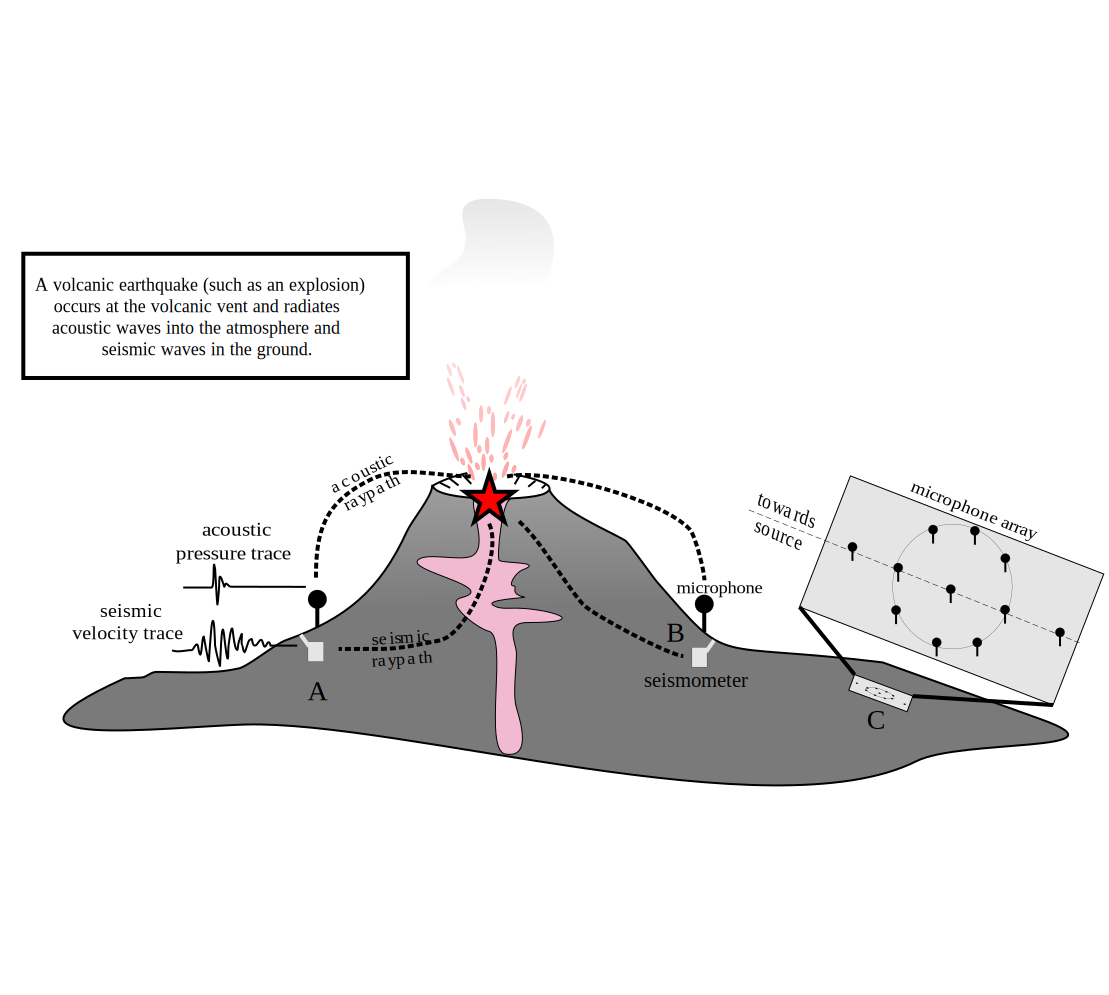
\includegraphics[width=0.9\hsize,clip=true,bb=20 470 540 770]{./figures/Cartoon2.pdf}
\end{center}
\caption{\small {\bf Sensor arrays for volcanic monitoring.}}
\label{fig-cartoon}
\end{figure*}

\subsection{Volcanic monitoring arrays and networks}

Volcanic sensors range from widely dispersed instrument networks to more
confined sensor arrays. An individual sensor station may consist of a
single sensor (e.g., seismometer or tilt sensor), or an array of several
closely-spaced ($10^2$ to $10^3$~m aperture) wired sensors, perhaps
of different types. Multiple stations may be integrated into a larger
network that is installed over an extended azimuthal distribution and
radial distance ($10^2$ to $10^4$~m) from the vent.  Data from the various
stations may be either recorded continuously or as triggered events and
the acquisition bandwidth depends upon the specific data stream. For
instance, seismic data is often acquired at 24-bit resolution at 100~Hz,
while tilt data may be recorded with 12-bit resolution at 1~Hz or less.

Sensor data at a station may be recorded locally or transmitted over
long-distance radio or telephone links to an observatory
located tens of kilometers from the volcano.  At the receiving site,
data is displayed on revolving paper helicorders for rapid general
interpretation and simultaneously digitized for further processing.
However, due to the expense and bandwidth constraints of radio telemetry,
high-quality, multi-channel data acquisition at a particular volcano is
often limited. These analog systems also suffer from signal degradation
and communication interference.

As a result, many scientific experiments use a stand-alone data
acquisition system at each recording station. 
The digitizer performs high-resolution 
analog-to-digital conversion from the wired sensors and stores data 
on a hard drive or Compact Flash card. However, these systems are
cumbersome, power hungry ($\approx
10$~Watts), and require data to be manually retrieved from the station
prior to processing. Depending on the size of the recording media,
a station may record several days or weeks' worth of data before
it must be serviced.

\subsection{Scientific and monitoring goals}

Volcanic monitoring has a wide range of goals, related to both
scientific studies and hazard monitoring. The type and configuration
of the instrumentation depends on the goals of a particular study.
Traditionally, dispersed networks of seismographs, which record 
ground-propagating elastic energy, are utilized to locate, determine the 
size of, and assess focal mechanisms (source motions) of earthquakes 
occurring within a volcanic edifice~\cite{Chouet03}. 
%Data from each 
%seismograph channel is usually recorded as a continuous time-series 
%of polarized local ground velocity.  
At least four 
spatially-distributed seismographs are required to constrain hypocentral 
(3D) source location and origin time of an earthquake, though
using more seismic elements enhances hypocenter resolution and the 
understanding of source mechanisms. Understanding spatial and temporal 
changes in the character of volcanic earthquakes is essential
for tracking volcanic activity, as well as predicting eruptions 
and paroxysmal events~\cite{McNutt96}. 

%well investigated through the 
%study of seismic network data and are critical for 

Another use of seismic networks is the imaging of the internal
structure of a volcano through tomographic inversion.  Earthquakes
recorded by spatially-distributed seismometers provide information
about propagation velocities between a particular source and receiver.
A seismically-active volcano thus allows for three-dimensional imaging
of the volcano's velocity structure~\cite{Benz96,Phillips91}. The
velocity structure can then be related to material properties of the
volcano, which may be used to determine the existence of a
magma chamber~\cite{Lees89,Moran99}.

Dense array configurations, with as many as several dozen
seismographs, are also an important focus of volcanic
research~\cite{Dietel89,Neuberg94}. Correlated seismic body and surface wave
phases can be tracked as they cross the array elements, enabling
particle motion and wavefield analysis, source back-azimuth calculations,
and enhanced signal-to-noise recovery.

\subsection{The role of infrasound}

Infrasonic signals are
becoming an increasingly important means by which to study volcanic
activity. An acoustic antenna, with three or more microphones that
record low-frequency sound pressure waves, are used for enhancing
signal-to-noise and discriminating the source of a volcanic
event~\cite{Johnson03}. In cases where the volcanic vent may not be
visible due to terrain or cloud cover, infrasonic signals can 
help differentiate eruptive activity from other sources of seismic 
signals such as mining operations or bovine ambulation. In volcanoes with multiple vents,
such as Stromboli, Italy, an array of acoustic sensors can
triangulate the precise location of individual eruptions~\cite{Ripepe02}.

Combining seismic and acoustic signals in a sensor array has great
potential for assessing eruption intensity and interpreting trends
in volcanic activity~\cite{Johnson04}.  Infrasonic signals have
also been used to track non-stationary sources~\cite{Yamasato97}
and to understand the weather-dependent velocity structure of the
atmosphere~\cite{Garces98}.

\subsection{Opportunities for wireless sensor networks}

Wireless sensor networks present new opportunities for volcanic
monitoring by offering increased scale and resolution.  As mentioned above,
analog radio telemetry has been used at volcanic monitoring stations
for some time. More recently, spread-spectrum digital modems have been
employed to transmit digital data from remote monitoring stations to an
observatory. For example, at Mount Erebus, Antarctica, a five-station
sensor array was installed that transmits real-time data over a FreeWave
modem~\cite{freewave} to a central PC that is connected to the Internet
over a geosynchronous satellite link~\cite{Aster04}.

However, these approaches are still limited in terms of the number of
individual channels (seismic, acoustic, etc.) that can be recorded at
each station and the communication bandwidth of the long-distance 
radio link. The number and placement of sensors at a station is limited by 
power requirements, cable length, and data recording capabilities.
For example, a typical data recorder supports only up to six 24-bit 
channels. The use of small, low-power, wireless sensor nodes can 
greatly benefit volcanic monitoring
studies, allowing researchers to deploy large sensor arrays in a
versatile fashion. A sensor array of tens of microphones or seismic
elements will improve spatial resolution and resilience to wind noise and
permit much more detailed analysis of received signals. Unlike a fixed data
logger, wireless sensor networks are 
reprogrammable, allowing researchers to experiment with signal processing,
compression, oversampling, and other techniques to improve the quality
of the data captured.

The use of wireless sensor networks in this context raises a number of
new challenges. The data rates from individual sensors ($\approx$ 100~Hz) 
are much higher than those in low data-rate applications, such as
environmental monitoring~\cite{mainwaring-habitat,gdi-ewsn04}. Therefore, new
approaches to managing bandwidth are required, since even a small 
number of sensors will saturate the wireless link. Rather than
sampling and transmitting data continuously, it is necessary to 
perform compression, correlation, or other processing of signals on
the sensor nodes themselves. In addition, sensor nodes must be tightly 
time synchronized to allow signals from each node to be compared. 



\section{Network Hardware and Architecture}
\label{evaluation-sec-architecture}

\begin{figure}[t]
\begin{center}
\includegraphics[width=1.0\hsize]{./3-evaluation/figs/node.pdf}
\end{center}
\caption{\textbf{Our wireless volcano monitoring sensor node.}}
\label{evaluation-fig-node}
\end{figure}

Our volcano monitoring sensor station consists of a Moteiv TMote
Sky~\cite{moteiv} wireless sensor network node, an 8~dBi~2.4GHz external
omnidirectional antenna, one or more seismometers, a microphone, and a custom
hardware interface board. An example node with components labeled is shown in
Figure~\ref{evaluation-fig-node}. The TMote Sky was designed to run
TinyOS~\cite{tinyos-asplos00}, and all of our software development made use
of this environment. We chose the TMote Sky for several reasons. The MSP430
microprocessor provides a large number of configurable ports, easily
supporting external devices, and the large amount of flash memory was useful
for buffering collected data.

We built a custom hardware board to integrate the TMote Sky with the
seismoacoustic sensors. The board features up to four Texas Instruments
AD7710 analog to digital converters (ADCs) providing up to 24~bits per
channel of resolution. Although the MSP430 microcontroller provides on-board
ADCs, they are unsuitable for our application. First, they provide only
16~bits of resolution while we required at least 20~bits. Second,
seismoacoustic signals require an aggressive filter centered around 50~Hz.
Due to the infeasibility of implementing such a filter using analog
components, it is usually approximated digitally, requiring several factors
of oversampling. To perform this filtering, the AD7710 is sampling at over
30~kHz while presenting an output word rate of 100~Hz. The high sample rate
and computation required by digital filtering are best delegated to a
specialized device.

Each sensor node was powered by a pair of alkaline D~cell batteries.
Anticipating a remote network location, D~cells provided the best combination
of low cost, high capacity, and ready availability, and are able to power a
node for over a week. Approximately 75\% of the power drawn by each node is
consumed by the sensor interface board, primarily due to the high power
consumption of the ADCs.

For sensors, nodes are fitted with either a Geospace Industrial GS-11
geophone --- a single-axis seismometer with a corner frequency of 4.5~Hz,
oriented in the vertical plane of motion --- or triaxial Geospace Industries
GS-1 seismometers with corner frequencies of 1~Hz, yielding separate signals
in each of the three axes. Both sensors are passive instruments: ground
motion generates a voltage which is amplified and digitized by the sampling
board. In addition, each node was attached to an omnidirectional microphone,
the Panasonic WM-034BY, which has been used in other infrasonic monitoring
studies~\cite{johnson-etal-04b}.

\subsection{Network Operation}

Given the current capabilities of wireless sensor network nodes, we set out
to design a data collection network meeting the application's scientific
requirements Before motivating and explaining our design we provide a
high-level overview of typical network operation.
Figure~\ref{evaluation-fig-architecture} outlines the main system components.

\begin{figure}[t!]
\begin{center}
\includegraphics[width=0.7\hsize]{./3-evaluation/figs/architecture.pdf}
\end{center}
\caption{\textbf{Schematic representation of our sensor network
architecture.}}
\label{evaluation-fig-architecture}
\end{figure}

Each node samples two or four channels of seismoacoustic data at 100~Hz,
storing the data in local flash memory. Nodes also transmit periodic status
messages and participate in routing and time-synchronization protocols. When
a node detects an interesting event, it routes a message to the base station
laptop. If enough nodes report an event within a short time interval, the
laptop initiates data collection, which proceeds in a round-robin fashion.
Between 30~and~60~s of data is downloaded from each node with a reliable data
collection protocol, ensuring that all buffered data from the event is
retrieved. When data collection completes, nodes return to sampling and
storing sensor data.

\subsection{Overcoming High Data Rates: Event Detection and Buffering}

When designing high data-rate sensing applications an important limitation of
current sensor network nodes is low radio bandwidth. IEEE 802.15.4 radios,
such as the Chipcon CC2420, have raw data-rates of around 30~kBps. However
overheads caused by packet framing, medium access control (MAC), and multihop
routing reduce the achievable data-rate to less than 10~kBps even in a
single-hop network. Because of the high data-rates involved (600-1200~Bps
from each node) it is infeasible to continuously transmit all data.

Rather, nodes are programmed to locally detect interesting seismic events and
transmit event reports to the base station. If enough nodes trigger in a
short time interval, the base station attempts to download the last 60~s of
data from each node. This forgoes continuous data collection for increased
resolution following significant seismic events, which include earthquakes,
eruptions, or long-period (LP) events, such as tremors. The download window
of 60~s was chosen to capture the bulk of the eruptive and earthquake events,
although many LP events can exceed this window (sometimes lasting minutes or
hours). To validate our network against existing scientific instrumentation,
our network was designed for high-resolution signal collection rather than
extensive in-network processing.

Sampled data is stored in the local flash memory of the node, which is
treated as a circular buffer. Each block of data is timestamped using the
local node time, which can later be mapped onto a global time, as explained
in Section~\ref{evaluation-subsec-timerectification}. Each node runs an
\textit{event detector} on locally-sampled data. Good event detection
algorithms produce high event-detection rates while maintaining small
false-positive rates. The sensitivity of the detection algorithm links these
two metrics: a more sensitive detector correctly identifies more events at
the expense of producing more false positives. We evaluate the performance of
our event detection algorithm further in
Section~\ref{evaluation-sec-eventdetection}.

\vfill\eject

The data set produced by our previous deployment at Tungurahua
volcano~\cite{volcano-ewsn05} aided in the design of the event detector. We
implemented a short-term average/long-term average threshold detector, which
computes two exponentially-weighted moving averages (EWMAs) with different
gain constants. When the ratio between short-term average and the long-term
average exceeds a fixed threshold, the detector fires. The detector threshold
allows nodes to distinguish between low-amplitude signals, perhaps caused by
distant earthquakes, and high-amplitude signals caused by nearby volcanic
activity.

When the event detector on a node fires it routes a small message to the base
station laptop. If the base station receives triggers from 30\% of the active
nodes within a given time window, the laptop initiates data collection from
the entire network, including nodes that did not report the event. This
global filtering prevents spurious event detections from triggering a data
collection cycle. Because each node can buffer only 20 minutes of eruption
data locally, and data collection from the entire network may exceed this
envelope (we found that fetching 60~s of data from 16 nodes takes over 1
hour) each node pauses sampling and reporting events until its data has been
uploaded.

\subsection{Reliable Data Transmission and Time Synchronization}
\label{evaluation-subsec-fetch}

\begin{figure}[t!]
\begin{center}
\includegraphics[width=0.7\hsize]{./3-evaluation/figs/fetchprotocol.pdf}
\end{center}

\caption{\textbf{Operation of the \texttt{Fetch} data transfer protocol.}
Fetch requests include the block and node ID and are propagated using a
reliable broadcast protocol. 256~byte blocks are fragmented into 8~chunks,
each sent in a single radio message. The sample transfer shows packets being
lost during transmission and a repair operation which requests any missing
chunks. Once all chunks for a block are received, the next block is
requested.}

\label{evaluation-fig-fetchprotocol}
\end{figure}

Extracting high-fidelity data from a wireless sensor network is challenging
for two primary reasons. First, radio links are lossy and frequently
asymmetrical. Second, low-cost crystal oscillators on sensor nodes have low
tolerances and so clock rates vary across the network. Much prior research
has focused on addressing these challenges.

We developed a reliable data-collection protocol, called \texttt{Fetch}, that
retrieves buffered data from each node over a multihop network.
Figure~\ref{evaluation-fig-fetchprotocol} provides an overview of the
protocol's operation. Samples are buffered locally in \textit{blocks} of
256~B, tagged with a sequence number and timestamp. During transmission each
requested block is fragmented into a number of \textit{chunks}, each sent in
a single radio message. The base station laptop retrieves a block by flooding
a request to the network using \texttt{Drip}, a variant of the TinyOS
\texttt{Trickle}~\cite{trickle} data-dissemination protocol. The request
contains the target node ID, the block sequence number, and a bitmap
identifying missing chunks in the block.

The target node replies by sending the requested chunks over a multihop path
to the base station. The routing tree is constructed using
\texttt{MultiHopLQI}, a variant of the TinyOS
\texttt{MintRoute}~\cite{awoo-multihop} routing protocol modified to select
routes based on the CC2420 Link Quality Indicator (LQI) metric. Link-layer
acknowledgments and retransmissions are used at each hop to improve
reliability. Retrieving one minute of stored data from a two-channel sensor
node requires fetching 206~blocks and can takes several minutes to complete,
depending on the quality of the multihop path and the node's depth in the
routing tree. We evaluate the performance of Fetch in more detail in
Section~\ref{evaluation-sec-performance}.

Scientific volcano studies require that sampled data be accurately
timestamped. In our case, a global clock accuracy of 1~ms was sufficient. We
chose to use the Flooding Time Synchronization Protocol (FTSP)~\cite{ftsp} to
establish a global clock across our network. The published accuracy of FTSP
is very high and the TinyOS code was straightforward to integrate into our
application. One of the nodes used a Garmin GPS receiver to map the FTSP
global time to GMT. Unfortunately, FTSP failures during our field deployment
made assigning accurate timestamps challenging, as documentented in
Section~\ref{evaluation-sec-timing}.

\subsection{Command and Control}

A feature missing from most traditional volcanic data acquisition equipment
is real-time network control and monitoring. The long-distance radio link
between the observatory and the sensor network allowed the laptop to monitor
and control the network's activity. Every 10~s, each node transmits a
\textit{status message} to the base station that includes its position in the
routing tree, buffer status, local and global timestamps, battery voltage,
and other information. In addition, the base station can issue a
\textit{command} to each node, instructing it to respond with an immediate
status message, start or stop data sampling, and set various software
parameters.

We developed a Java-based GUI for monitoring the network's behavior and
manually setting parameters, such as sampling rates and event detection
thresholds. In addition, the GUI was responsible for controlling data
collection following a triggered event, moving significant complexity out of
the sensor network. All packets received by the laptop from the sensor
network were logged, facilitating later analysis of the network's operation.

The GUI also displayed a table summarizing network state, based on the
periodic status messages transmitted by each node. Each table entry included
the node ID; local and global timestamps; various status flags; the amount of
locally-stored data; depth, parent, and radio link quality in the routing
tree; and the node's temperature and battery voltage. This functionality
greatly aided sensor deployment, as a team member could rapidly determine
whether a node had joined the network and the quality of its radio
connectivity.

\section{Policy Modules}
\label{lance-sec-policies}

Policy modules provide an interface through which applications can tune the
operation of the Lance optimizer. Since policy modules are loaded into the
system at the base station, they can be modified at any time without
necessitating reprogramming of the sensor nodes themselves. In this section
we provide a general discussion of policy modules and examples of policies
that can be implemented using this feature.

\subsection{Definitions}

A policy module is an application-supplied function that takes as input an
ADU $a_i = \{ i, n_i, t_i, d_i, \bar{c}_i, s_i, v_i \}$ and produces a new
ADU $a'_i$ with a possibly modified value $v'_i$. Policy modules run at the
base station, can maintain internal state, and operate with global knowledge
of the ADUs stored in the network.

\vfill\eject

A series of policy modules $\{m_1, m_2, ... m_n\}$ are composed into a linear
chain, which is passed the ADU information extracted from the ADU summary
messages received at the base station. The first policy module in the chain
is responsible for assigning the initial value $v_i$ to the ADU based on the
summary information $s_i$ calculated by the sensor node. The final ADU value
produced by the chain is used as input to Lance's optimizer for the purpose
of scheduling ADUs for download.

Lance requires that policy modules be efficient in that they can process the
stream of ADU summaries received from the network in real time. In practice
this is not difficult to accomplish, as the rate of ADU summary reception is
modest, and the base station (typically a PC or laptop) is assumed to have
adequate resources. For example, a 100-node network with an ADU size of
60~s would receive an ADU summary every 600~ms. Typical policy modules
take a small fraction of this time to run.

One of the main benefits of policy modules is that they permit significant
changes to the network's behavior \textit{without requiring changes to the
node-level summarization function}. Changing the latter would typically
involve reprogramming sensor nodes. In the field, it is often undesirable to
reprogram the network except when absolutely necessary, and in many cases it
is difficult to reach sensor nodes physically once deployed. Although systems
such as Deluge~\cite{deluge} permit over-the-air reprogramming, any changes
to the sensor node software could result in unexpected failures that can be
very difficult to debug without manual intervention. On the other hand,
introducing new policy modules at the base station is relatively
straightforward and can be quickly reversed without risking sensor node
failures.

\subsection{Example policy modules}

\begin{table}[t]
\label{lance-fig-policymodules}
\begin{center}
\begin{tabular}{|l|l|} \hline
\textit{Policy module} & \textit{Description} \\ \hline
\texttt{filter} & Set ADUs below threshold to zero value \\
\texttt{boost} & Set ADUs above threshold to max value \\
\texttt{timespread} & Dilate ADU values across time \\
\texttt{spacespread} & Dilate ADU values across space \\
\texttt{adjust} & Add or subtract offset to ADU value \\
\texttt{smooth} & Apply low-pass filter to remove noise \\
\texttt{debias} & Median filter DC debiasing \\
\texttt{correlated} & Boost values for correlated events \\
\texttt{costfilter} & Filter ADUs above cost threshold \\
\texttt{valuefilter} & Filter ADUs below value threshold \\ \hline
\end{tabular}
\end{center}

\caption{\textbf{Standard policy modules provided by Lance.}}

\label{lance-sec-example-policies}
\end{table}

Policy modules can be used to encapsulate a wide range of data collection
goals, and make it easy to customize Lance's behavior for specific
applications. We provide a standard toolkit of general-purpose policy
modules, summarized in Figure~\ref{lance-fig-policymodules}. Application
developers are free to implement their own modules as well. By composing
modules in a linear chain, it is easy to implement various behaviors without
requiring a general-purpose ``policy language.''

\begin{itemize}

\item \textbf{Value thresholding:} \texttt{filter} is perhaps the simplest
example of a policy module that filters out ADUs with a value below a given
threshold $T$ by setting their values to zero. Setting $v'_i = 0$ prevents
an ADU from being considered for download by the optimizer. This type of
filtering can be used to force a drop of low-valued data. Conversely, the
\texttt{boost} policy module sets the value for an ADU above a given
threshold to the maximum value, ensuring it will be downloaded as soon as it
is feasible.

\item \textbf{Value adjustment and noise removal:} Policy modules can be used
to remove the effects of noise or correct for node-level value bias, for
example, based on poor sensor calibration or differences in site response.
Moreover, since each node computes the ADU summary based only on local sensor
data, it may be necessary to normalize the ADU values in order to compare
values across nodes.

\hspace{0.25in} \texttt{adjust} adds or subtracts a node-specific offset to
each ADU value to correct for differences in sensor
calibration.\texttt{smooth} applies a simple low-pass filter on the raw ADU
values to remove spikes caused by spurious sensor noise. Likewise,
\texttt{debias} is intended to remove sensor-specific DC~bias from the ADU
values. \texttt{debias} computes the median ADU value for a given node over a
time window. It then subtracts the median from each ADU value before passing
it along to the next module in the chain.

\hspace{0.25in} Likewise, when a sensor network contains multiple sensors
with varying sensitivity, it is natural to prioritize data from more
sensitive instruments. In cases where networks are deployed to monitor fixed
physical phenomena, it may be desirable to prioritize data from nodes located
close to the phenomena being observed. The \texttt{adjust} module can be used
to scale raw ADU values based on a sensor's location, SNR, or other
attributes.

\item \textbf{Value dilation:} Another useful policy is to dilate a high (or
low) ADU value observed in one ADU across different ADUs sampled at different
times or different nodes. This can be used to achieve greater spatial or
temporal coverage of an interesting signal observed at one or more nodes. The
\texttt{timespread} detects ADUs with a value above some threshold $T$ and
assigns the same value to those ADUs sampled just before and just after.

\hspace{0.25in} Likewise, the \texttt{spacespread} module groups ADUs from
multiple nodes into time windows and assigns the maximum ADU value to all
ADUs in that window. Define a window $W(t,\delta)$ as the set of ADUs such
that $t-\delta \leq t_i \leq t+\delta$ where $t$ represents the center of the
window and $\delta$ the window size. \texttt{spacespread} determines the
maximum ADU in the window $v^* = \arg_{i \in W} \max v_i$ and sets $v'_i =
v^{*}$ for each ADU in $W$.

\vfill\eject

\item \textbf{Correlated event detection:} The \texttt{correlated} module is
used to select for ADUs that appear to represent a correlated event observed
across the entire sensor network. \texttt{correlated} counts the number of
ADUs within a time window $W(t,\delta)$ with a nonzero ADU value. If at least
$k$ ADUs meet this criterion, we assume that there is a correlated stimulus,
and the values for all ADUs in the set are passed through. Otherwise, we
filter out the ADUs in the window by setting $v'_i = 0$ for each ADU in $W$.

\hspace{0.25in} As an example of composing policy modules to implement an
interesting behavior, consider the chain \[
\mathit{filter}(T)\rightarrow\mathit{correlated}(k)\rightarrow\mathit{spacespread}
\] This policy filters incoming values, rejects time-correlated sets with
fewer than $k$ ADUs above the threshold, and assigns the max value across the
set to all ADUs. This can be useful in systems that wish to perform
collection of time-correlated data, but avoid spurious high-value data from a
few nodes. This policy is similar to the earthquake detector discussed in
Section~\ref{evaluation-sec-eventdetection}.

\item \textbf{Cost-based filtering:} Lance's optimizer considers both the
cost of ADUs as well as their application-assigned values when making
download scheduling decisions. The cost vector $\bar{c}_i$ is also available
to the policy module chain, allowing policy modules to perform their own
adjustments to the ADU value according to cost, permitting applications to
augment Lance's own policies for energy scheduling. For example, the
\textit{costfilter} policy module filters out ADUs with a total energy cost
$\sum_j c_i^j$ greater than some threshold; this ensures that the network
avoids expending an arbitrary amount of energy to download a given ADU
(regardless of its data value). Policy modules give applications a great deal
of control over energy usage to complement Lance's own energy scheduling
policy.

\item \textbf{Value-based filtering:} Lance's policy modules can store and
utilize history when modifying ADU values. This can be useful when \textit{a
priori} information about the expected ADU value distribution is known. For
the volcano monitoring example, traces of activity at the volcano of interest
may be available before deployment. These may be used to produce a
distribution of ADU values based on the activity levels seen during that time
period. Lance can use this distribution to decide how interesting a
particular ADU is in the context of a longer period of activity.

\hspace{0.25in} This can be particularly helpful as a way of bootstrapping
the system. Without seeding it in this way, if Lance begins running while the
volcano is quiet it will greedily begin downloading the highest-value ADUs
available despite the fact that these do not in fact contain interesting
data, wasting energy that could be saved and used later. Instead, it could
use the \textit{valuefilter} policy module with a filter threshold chosen
based on the expected ADU distribution, perhaps chosen to ADUs with values in
the top percentile. The filter threshold can also be adjusted online based on
the value distribution as ADUs are sampled.

\end{itemize}

\subsection{Interaction with ADU Summary Delivery}

The policy module chain is invoked each time a new summarization message
arrives at the base station. Once the application has assigned an initial
value, the ADU is passed to the policy module chain for processing. Note that
ADU inputs may stall along the policy module chain, or be grouped by policy
modules, so that inserting a new ADU into the chain may produce that ADU as
output, may not produce an output, or may produce a different ADU or set of
ADUs as output.

Note that policies modules like \texttt{correlated} which rely on information
from multiple nodes have to cope with delayed or missing information
resulting from dropped summarization messages. These policy modules will
usually hold sets of ADUs while awaiting members that have not yet arrived,
and then release a whole group at once after they have heard from a complete
set of nodes or a timeout occurs. When data is missing or delayed, we expect
different policy modules to respond differently. Some may choose to compute
their functions over incomplete sets of ADUs, others may not and either set
the values to zero (inhibiting download) or leave them unchanged.

Depending on the sensitivity of the policy modules in use to missing data,
different summarization message formats can be used. For our experiments we
send summarization messages each time an ADU is sampled, but which contain
the last $k$ ADU summaries (up to the maximum packet size). This ensures
that, if one is dropped, the next will contain the missing information. Other
applications may want to reduce the summarization overhead further by not
sending summarization messages each time an ADU is produced, with resulting
higher delays in policy modules like \texttt{correlated}.

\section{Adaptating Applications to Lance}
\label{lance-sec-adaptation}

As mentioned, the Lance approach grew out of challenges emerging from our
2005 field deployment at Reventador. Although this system was successfully
deployed, it exhibited several deficiencies which led to a significant loss
of data~\cite{volcano-osdi06}.

The first problem is that the decision used to download a given signal was
based on a simplistic binary approach, based on the event-detection algorithm
running on each node. As a result, the system could not prioritize certain
events over others. The event-detector logic used a simple threshold scheme,
and as reported in~\cite{volcano-osdi06}, the threshold was set too low,
causing the network to trigger on less than 5\% of the actual seismic events.

The second problem was that following each trigger, the network initiated a
\textit{nonpreemptive} download from every node in the network in a
round-robin fashion. This policy caused the system to devote resources to
downloading small precursor earthquakes that immediately preceded larger
eruptions~\cite{volcano-osdi06}. As a result, many such larger events were
not captured.

Finally, our 2005 system made no attempt to manage energy. As a result, the
expected lifetime of the network is only about a week (using D-cell
batteries), necessitating frequent battery changes over a long deployment.
Clearly, this system could benefit from a prioritized approach to download
management that also considers energy costs to increase lifetime.

\subsection{Volcano Monitoring}
\label{lance-subsec-volcano}

To address these problems, we reimplemented our previous volcano monitoring
system using Lance. Many of the components of the original system, such as
multihop routing, time synchronization, reliable download protocol, and flash
storage interface, remained unchanged. The node-level event detector was
replaced by an ADU summarization function, as described below. The base
station code for responding to correlated events was replaced with Lance's
optimizer and policy modules. Our deployment of the completed system at
Tungurahua volcano in August 2007 is discussed in
Section~\ref{lance-sec-deployment}.

The original system was intended to detect correlated seismic events from
across the network and download data from all nodes, regardless of whether
every node detected the event. This was based on a simple event detector that
computes two exponentially-weighted moving averages (EWMA) of the seismic
signal, with different gain settings; one EWMA represents the short-term
average and the other the long-term average. When the ratio between these two
averages exceeds a threshold, an event detection message is sent to the base
station. Subsequent triggers are suppressed for a short duration afterwards.

This policy is straightforward to implement in Lance by using the ``ratio of
two averages'' as the node-level summarization function. Rather than
performing thresholding at the node level, we report the maximum ratio over
the ADU as its value, allowing Lance to prioritize different events. The base
station's policy modules are configured as shown in
Section~\ref{lance-sec-example-policies}, using a chain of \texttt{filter},
\texttt{correlated}, and \texttt{spacespread} to implement the equivalent of
the event triggering policy used in the original system. Note that the Lance
version of the system differs from the original in that download management
is value-driven rather than FIFO. Also, Lance can download ADUs from
different events out of order, avoiding the nonpreemptive download problems
of the earlier system.

While our original system was designed to capture short earthquakes, were
also interested in determining whether Lance could be used to capture
different types of volcanic activity. For this, we make use of the Real-Time
Seismic Amplitude Measurement (RSAM)~\cite{rsam}, which computes the average
seismic amplitude over a given time window. Intuitively, RSAM measures the
total amount of ground shaking caused by earthquakes and tremor, and is often
used by volcano observatories to characterize the overall level of seismic
activity.

Different summarization functions and policy modules can be used to implement
a wide range of geophysical monitoring systems with Lance. For example, a
hazard monitoring system could be configured to periodically report RSAM
values for all sensor nodes and download only the strongest events for
further analysis. By limiting downloads to those ADUs with RSAM above some
threshold, energy can be saved. In contrast, a scientific study that wishes
to perform earthquake localization~\cite{aki-richards-80} or tomographic
inversion~\cite{lees-lindley-94} would prefer to download only small
earthquakes with clearly delineated onsets, which can be used to determine
the velocities of seismic waves. Likewise, a researcher studying explosive
events would prefer to download only seismic events with a corresponding
infrasonic component, since non-explosive earthquakes should not generate any
infrasound.

\subsection{Other Application Domains}

We believe that Lance can be used to benefit many applications that make use
of high-resolution signals delivered over a bandwidth-limited wireless
network. These applications require high data rates, precluding continuous
data collection, and rely on classification techniques to determine which
signals to download. Three examples follow.

\begin{enumerate}

\item \textbf{Structural monitoring:} Structural monitoring systems collect
vibration waveforms from a building, bridge, or other structure in order to
study structural properties and seismic response. In previous
systems~\cite{netshm-emnets05,ggb-ipsn07}, data collection has been triggered
manually or on a simple periodic schedule. Instead, Lance can be used to
prioritize signals following an earthquake or forced excitation of the
structure, similar to the EWMA and RSAM functions described earlier. To save
energy, the system could choose a subset of nodes from which to download data
to achieve a good spatial distribution across the structure. The size of the
subset could be chosen depending on the strength of the excitation. In
addition, policy modules can be used to perform periodic downloading of ADUs
from each sensor for calibration, as well as to determine whether each sensor
is still functioning properly.

\textbf{Animal habitat monitoring:} Habitat monitoring applications that
deploy high-bandwidth sensors, such as microphones or cameras, are good
candidates for prioritized data extraction. An example application may
attempt to download interesting audio signals facilitating offline species
classification or localization~\cite{girod-ipsn07}. The summarization
function could involve either a triggered event detector, an audio waveform
classifier, or motion detector from a series of camera images~\cite{cyclops}.

At the base station, policy modules can use offline knowledge of node
positions to modify the initial ADU value. One approach might enhance spatial
coverage by prioritizing data collection from nodes nearby the source of the
signal. Another could reject noise by deprioritizing signals detected by only
one node. For example, if fewer than three nodes report an audio event, it is
impossible to perform acoustic localization and Lance need not waste
bandwidth on the signal. Policy modules can take other metrics into account
as well, such as the SNR of the recorded signal or the time of day (e.g.,
reducing confidence in camera images taken at night).

\XXXnote{GWA: Move discussion of Mercury to later in the chapter.}

\item \textbf{Medical monitoring:} Another application domain that we are
exploring is motion analysis of patients with movement disorders, such as
Parkinson's Disease~\cite{parkinsons-embs07}. In this context, up to ten
sensor nodes equipped with triaxial accelerometers and gyroscopes are placed
on the patient's limb segments (two each on the arms and legs plus one each
on the torso and waist), collecting high-resolution data at rates up to
100~Hz or more. The goal is to capture data from the body sensor network
during periods of dyskinesia (abnormal movements) or bradykinesia (slowness
of movement) associated with the disease. The base station will typically be
a laptop located in the home, and as such will experience a wide variation in
bandwidth to the body sensor network (including disconnections), depending on
the patient's location.

Use of low-power wireless sensors keeps the size and weight of each device
down: for example, the wearable sensor node described
in~\cite{parkinsons-embs07} measures $44 \times 20 \times 13$~mm and weighs
just 10~g. While the sensor network is not spatially distributed, and all
nodes are within a single radio hop of each other, the data rates greatly
exceed the radio channel bandwidth: a single node will consume more than a
quarter of the best-case radio capacity, assuming no protocol overhead or
retransmissions.

Following our deployment at Tungurahua Volcano in 2008 we adapted the Lance
system to support this medical monitoring application, resulting in a system
called Mercury~\cite{mercury-sensys09}. Mercury makes use of Lance to drive
the energy and bandwidth management. Each sensor node computes a series of
high-level \textit{features} from the raw sensor data, such as peak
amplitude, maximum entropy, and RMS. The node prioritization function assigns
higher priority to features appearing to represent abnormal movement. The raw
signal is also stored as separate ADUs with lower priority than the features,
allowing Lance to restrict downloads of the raw data to periods with a strong
radio link to the sensors. During periods of disconnection, nodes will buffer
ADUs for later transmission; the wearable sensors we are using support a
large (up to 2~GByte) flash memory for this purpose. Policy modules at the
base station estimate the available bandwidth to the body sensors, based on
radio link quality, and prioritize downloads accordingly.

\end{enumerate}

\section{Prototype Implementation}
\label{sec-implementation}
\label{sec-implementation-nsm}

We have implemented Lance in TinyOS 2.x~\cite{tinyos-asplos00} for 
TMote~Sky and iMote2 sensor nodes. The TMote~Sky features a
1~MB flash memory (ST~M25P80) divided into 16~sectors of 64~KB each.
Our current prototype matches the ADU size to the sector size to
simplify storage management, but this is not a fundamental limitation
in the design. Sensor nodes participate in a multihop spanning-tree 
protocol rooted
at the base station; we use the Collection Tree Protocol provided with
TinyOS~2.0 for this purpose. Nodes send a periodic storage summary to the
base station. To improve reliability, we use a
sliding window approach in which each summary includes information on
the last 5~ADUs recorded by the node. The node prioritization function
is implemented as an application-supplied NesC component conforming to
a simple API. Our prototype uses our own Fetch~\cite{volcano-osdi06}
reliable transfer protocol, although it would be straightforward to
replace this with another protocol such as Flush~\cite{flush-sensys07}.

The Lance download manager runs at the base station and receives
data from the network via a ``gateway node'' connected to the base
station by a serial cable or radio modem.  The download manager is 
implemented in Perl and makes use of several external utilities for
reading and parsing storage summary packets and sending download
requests to the network. Policy modules are implemented as separate
UNIX processes (which can be in any language; we typically use Perl) 
that read storage summaries on {\tt stdin} and produce modified
storage summaries on {\tt stdout}. A simple configuration script is
used to compose multiple policy modules into a pipe. We find that
using standard scripting languages and UNIX utilities makes it very
easy to implement a range of policy modules.
A suite of Python utilities for logging, data visualization, and 
managing the network through a GUI are also provided.

\section{Evaluation}
\label{lance-sec-evaluation}

\begin{figure}[t]
\begin{center}
\includegraphics[width=1.0\hsize]{./4-lance/figs/linear.pdf}
\end{center}

\caption{\textbf{Per-node distribution of ADU value and energy usage for the
linear simulation experiment.} The top graph shows the amount of data value
downloaded from each node, while the bottom graph breaks down the amount of
energy used by each node into the downloading, routing and overhearing
components. Node~1 is closest to the base station.}

\label{lance-fig-linear}
\end{figure}

\begin{figure}[t]
\begin{center}
\includegraphics[width=1.0\hsize]{./4-lance/figs/error.pdf}
\end{center}

\caption{\textbf{Effect of cost vector error on optimality.} The optimization
process is guided by the cost vectors, but predicting the energy cost of
operations before they are performed can be difficult. Here we show the
impact of introducing a degree of error into the cost vectors used by the
optimizer. As can be seen, we can tolerate a relatively high degree of error,
as long as the shape of the cost vector does not change.}

\label{lance-fig-error}
\end{figure}

This section presents a careful evaluation of Lance conducted along several
lines. Using a high-level system simulator and synthetic data sets, we
evaluate the three scoring functions described in
Section~\ref{lance-subsec-optimizer}. We motivate the use of the
\textit{cost-bottleneck} scoring function and demonstrate that it performs
better than simpler alternatives. Next, we look at the effect of varying
parameters such as download bandwidth and network lifetime, as well as the
impact of errors in the cost vectors. We also present results from
experiments run on a 50-node sensor network testbed using realistic data
sets.

\subsection{Metrics and Methodology}

\begin{figure}[t]
\begin{center}
\includegraphics[width=1.0\hsize]{./4-lance/figs/crossover.pdf}
\end{center}

\caption{\textbf{Crossover between bandwidth and energy constraint dominance
as lifetime is varied.} This graph shows the transition between bandwidth and
energy constrained regions for an optimal system. The right axis shows the
percent of energy consumed by the most highly-drained node, and the left axis
shows the amount of time spent downloading.}

\label{lance-fig-crossover}
\end{figure}

As stated in Section~\ref{lance-sec-problem-definition}, the high-level goal
of Lance is to download a set of ADUs maximizing the total value subject to
energy and bandwidth constraints. The \textit{optimal} solution is defined as
the solution to the multidimensional knapsack problem, which yields a set of
downloaded ADUs $\mathcal{O} = \{a_1, a_2, ... a_n\}$ that maximize data
value subject to bandwidth and energy constraints. The total data value of
the optimal solution $\hat{v}(\mathcal{O}) = \sum_{a_i \in \mathcal{O}} v_i$.
Recall that computing the optimal solution requires \textit{a priori}
knowledge of all of the ADU values sampled by the network over time. We
define \textit{optimality} as the fraction of the data value downloaded by
Lance compared to the optimal solution. That is, given a set of downloaded
ADUs $\mathcal{L}$ with total data value $v(\mathcal{L})$, we define
optimality as $v(\mathcal{L}) / \hat{v}(\mathcal{O})$.

We begin by presenting results based on a realistic system simulator that
allows us to quickly vary parameters such as ADU data value distribution,
network topologies, download speeds, energy costs, and target lifetimes. We
also present results from Lance running on MoteLab~\cite{motelab}, a sensor
network testbed deployed over 3~floors of the Harvard EECS building. Our
simulation experiments use a 10-node linear topology as well as a 25-node
realistic tree topology shown in Figure~\ref{lance-fig-topology}(a).
Both topologies use per-node ADU download speeds based on empirical
measurements taken using the testbed. In our experiments, the ADU size is
36~KB and each node samples one ADU every 60~s (or 600~Bps of data).

We draw ADU values from several distributions in an attempt to understand
Lance's behavior as the properties of the sampled data change. Three value
distributions are used: uniform random, exponentially distributed, and Zipf
with exponent $\alpha = 1$. We also make use of an ADU value distribution
based on a 6~hour seismic signal collected at Reventador Volcano, Ecuador in
2005. Except where stated, no policy modules were used. In order to compute
optimal solutions, we frame the problem as a multi-dimensional knapsack
problem as previously described and solve the resulting instance using
\texttt{lpsolve}.

The energy costs for various operations are modeled as follows. The
background current drain of each node is set to 2~mA, based on empirical
measurements of a TMote~Sky sensor node performing high-data-rate sampling
and storing to flash. We also measured the current consumption to download an
ADU from a sensor node, and derived the energy costs for downloading ($E_d =
17.6$~mA/s), routing ($E_r = 16.9$~mA/s), and overhearing ($E_o = 2$~mA/s).
Our experiments assume that each node can only overhear its parent in the
routing tree; developing more detailed overhearing models is the subject of
future work. Computing the components of the cost vector for a particular ADU
is done by multiplying the current consumption by the ADU download time for
each node either downloading, routing, or overhearing the transmission.

\subsection{Effectiveness of Scoring Functions}
\label{lance-sec-eval-heuristics}

\begin{figure}[t]
\begin{center}
\includegraphics[width=1.0\hsize]{./4-lance/figs/motivationexample.pdf}
\end{center}

\caption{\textbf{Example simple download problem.}}

\label{lance-fig-simple}
\end{figure}

\begin{table}[t]
\begin{center}
\begin{tabular}{|l|l|ccc|}
\hline
& & \multicolumn{3}{|c|}{Scoring Functions} \\ \hline
& & Value & Cost & Cost \\
Distribution & Lifetime & Only & Total & Bottleneck \\ \hline
\multirow{3}{*}{Uniform} & 4 months & 62.4\% & 90.5\% & \textbf{93.2\%} \\
& 11 months & 43.4\% & 68.0\% & \textbf{96.9\%} \\
& 18 months & 44.6\% & 49.0\% & \textbf{90.0\%} \\ \hline
\multirow{3}{*}{Exponential} & 4 months & 83.9\% & 85.1\% & \textbf{88.0\%}
\\
& 11 months & 70.4\% & 82.0\% & \textbf{93.0\%} \\
& 18 months & 67.2\% & 72.8\% & \textbf{91.2\%} \\ \hline
\multirow{3}{*}{Zipfian} & 4 months & 84.7\% & \textbf{91.4\%} & 87.1\% \\
& 11 months & 63.8\% & 91.1\% & \textbf{96.2\%} \\
& 18 months & 53.1\% & 86.9\% & \textbf{93.8\%} \\ \hline
\end{tabular}
\end{center}

\caption{\textbf{Optimality of different scoring functions.} This table
summarizes simulation results evaluating the three different scoring
functions. Results are shown for several different lifetime targets and value
distributions. \textit{cost-bottleneck} out-performs the others in almost all
cases.}

\label{lance-fig-table}
\end{table}

We begin by evaluating the three scoring functions described
Section~\ref{lance-subsec-optimizer}. We want to see which is the most able
to approximate the optimal solution across a range of target lifetimes and
ADU distributions. As discussed earlier we expected the \textit{value-only}
scoring function, without considering the energy or bandwidth overhead of
downloading each ADU, to consume more energy downloading high-valued ADUs
when it could have increased the total data value by downloading several
slightly less-highly valued ADUs with lower costs. The \textit{cost-total}
scoring function incorporates a notion of cost, but will tend to favor nodes
closer to the base station at the expense of high-valued ADUs that are more
routing hops away. The \textit{cost-bottleneck} scoring function should
strike a balance between the two, since it considers only the most
significant cost vector component when ranking ADUs.

To develop intuition, consider the simple download problem shown in
Figure~\ref{lance-fig-simple}. The figure shows the network topology with the
energy required to reliably use each link labeled. Note that since we assume
that node radios are left on throughout the transfer the cost to route data
towards the sink is driven by the worst link along the path. links. So
Nodes~2 and 1 in the figure shown will have a cost of 100~units to route each
packet for Node~3 due to the poor link between Nodes~2 and 3. Three ADUs are
available in the network, one at each of nodes 1, 2, and 3, and the values of
each are labeled. Also assume that Nodes 1, 2 and 3 have 300, 600 and 2,000
units of available energy, respectively.

The question is: given the battery states, download costs, and values of each
ADU, which ADU should Lance download? To summarize the three ADUs available:

\begin{itemize}

\item \textbf{$ADU_1$}: located at Node~1 with value $v_1 = 10$ and cost vector
$\bar{c}_1 = \left[10, 0, 0\right]$. Note we are not considering the cost at the base
station, which we assume to be powered.
\vspace*{-0.1in}
\item \textbf{$ADU_2$}: located at Node~2 with value $v_2 = 20$ and cost vector
$\bar{c}_2 = \left[15, 15, 0\right]$.
\vspace*{-0.1in}
\item \textbf{$ADU_3$}: located at Node~3 with value $v_3 = 40$ and cost vector
$\bar{c}_3 = \left[100, 100, 100\right]$.

\end{itemize}


For this example, the three scoring functions make three different choices:

\begin{itemize}

\item \textbf{\textit{value-only}} will choose the ADU with the highest
value, $ADU_3$, regardless of the energy impact on the network.

\item \textbf{\textit{cost-total}} will compute the total cost of each ADU
and use that to weight the ADU's value. For this set of ADUs, $ADU_1$ has the
best ratio of value to total cost of the three choices: $0.1$, $0.066$ and
$0.013$ respectively.

\item \textbf{\textit{cost-bottleneck}} will first compute the bottleneck
node for each ADU by determining which node will be the most impacted by
downloading it. In this case, Node~1 is the bottleneck node for all three
ADUs, since it must devote 3.3\% of its remaining energy to $ADU_1$ (versus
0\% for Nodes~2 and 3), 5.0\% to $ADU_2$ (versus 2.5\% for Node~2 and 0\% for
Node~3), and 33\% to $ADU_3$ (versus 16\% for Node~2 and 5\% for Node~3).

\hspace{0.25in} Identifying the bottleneck cost causes
\textit{cost-bottleneck} to choose $ADU_2$, which has the best ratio of value
to  bottleneck cost (or cost to Node~1 in this case): $0.13$ versus $0.1$ for
$ADU_1$ and $0.04$ for $ADU_3$.

\end{itemize}

To convince ourselves that the \textit{cost-bottleneck} scoring function has
made the correct choice for this simple example, imagine that we can
repeatedly download ADUs with these values from each node in the network
until nodes run out of energy. We can download 30 copies of $ADU_1$ for a
total value of 300, 20 copies of $ADU_2$ for a total value of 400, or 3
copies of $ADU_3$ for a total value of 120. $ADU_2$ is the correct choice.

In many cases the node connecting the network to the powered sink quickly
becomes the bottleneck node, since all network traffic must be routed through
it. Figure~\ref{lance-fig-linear} shows simulation results using the 10-node
linear topology with exponentially-distributed ADU values, and a target
lifetime of 3~months. Nodes are numbered in increasing distance from the base
station. The graph confirms the intuition behind the scoring function
behavior. \textit{value-only} downloads roughly equal value from each node,
but fails to match the optimal performance. \textit{cost-total} downloads
more data from nodes near the sink. \textit{cost-bottleneck} comes close to
matching the optimal solution, retrieving over 99\% of the value retrieved by
the optimal solution. The smooth fall-off in the amount of value downloaded
from each node is a result of the decaying transfer speeds as the protocol
must communicate with nodes deeper in the tree. Node~1 is always the
bottleneck node during this experiment.

\begin{figure}[t]
\begin{center}
\includegraphics[width=1.0\hsize]{./4-lance/figs/zipfian.pdf}
\end{center}

\caption{\textbf{Scoring function performance on Zipfian distribution.} The
\textit{cost-bottleneck} scoring function outperforms the other two across a
range of lifetime targets.}

\label{lance-fig-zipfian}
\end{figure}

\begin{figure}[t]
\begin{center}
\includegraphics[width=1.0\hsize]{./4-lance/figs/speeds.pdf}
\end{center}

\caption{\textbf{Effect of varying download bandwidth.} Lance maintains a
high degree of optimality as the per-node download bandwidth is varied. Here
results are shown for the three synthetic distributions across a 25~node tree
topology and the \textit{cost-bottleneck} scoring function. Note that the
$y$-axis starts at 90\%.}

\label{lance-fig-speeds}
\end{figure}


Table~\ref{lance-fig-table} summarizes simulation results from a variety of
different lifetimes and value distributions, run on the 25-node tree
topology. The table shows that the \textit{cost-bottleneck} scoring function
outperforms the other two in most cases, with optimality values between
87.1\% and 96.9\%. The one exception is the 4-month Zipfian data set, where
\textit{cost-total} slightly outperforms \textit{cost-bottleneck}.
Figure~\ref{lance-fig-zipfian} shows the effect of varying the network's
target lifetime, using the 25-node tree topology and a Zipfian data value
distribution. As the figure shows, the \textit{cost-bottleneck} scoring
function maintains a high degree of optimality as the network bandwidth
changes.

\vfill\eject

To illustrate the effect of varying lifetime targets in more detail,
Figure~\ref{lance-fig-crossover} shows how the optimal solution transitions
between bandwidth-dominant and energy-dominant constraints as the target
lifetime increases. At low lifetime targets, the system is bandwidth
constrained and cannot download data fast enough to exhaust the nodes'
batteries. At high lifetime targets, the system is energy constrained and
cannot download continuously without exhausting the nodes' batteries.

\subsection{Bandwidth Adaptation}
\label{lance-sec-eval-params}

Next, we evaluate the impact of varying the download bandwidth in
Figure~\ref{lance-fig-speeds}, using the 25-node tree topology and the
\textit{cost-bottleneck} scoring function. We vary the per-node download
bandwidth from 128~to~2048~Bps and peg the target lifetime at 8~months.
As the figure shows, Lance performs well across the range of bandwidths, with
optimality greater than 97\% in all cases.

\subsection{Effect of Cost Vector Error}

Our last simulation study evaluates the effect of introducing errors into
estimated download cost. This experiment uses the 25-node topology,
\textit{cost-bottleneck} scoring function, and an exponential data
distribution. As described in Section~\ref{lance-subsec-costestimation}
estimating the cost of performing different operations \textit{a priori} can
be difficult. As shown in Figure~\ref{lance-fig-error}, even a 40\% error in
each component of the cost vector $\bar{c}_i$ for a given ADU only degrades
optimality by approximately 15\%. We conclude that accurate estimations of
download costs are not strictly necessary to achieve good performance.

Note that \textit{cost-bottleneck} depends on the ability to correctly
identify the bottleneck node. This is critical as that is the node whose cost
will be used to weight the value. In general we cannot compute the cost
perfectly \textit{a priori}, as described above. If two nodes have similar
values of $B(a_i,n)$ during the calculation of the bottleneck score, it is
possible that, assuming some error in the cost vector $\bar{c}_i$, we will
identify the wrong bottleneck and weight the value incorrectly. If the errors
are evenly distributed then over time we expect these mistakes to even out.
However, if there is a persistent miscalculation affecting one or both of the
nodes then we may repeatedly identify the wrong node as the bottleneck,
reducing optimality.

\subsection{Testbed Experiments}
\label{lance-sec-eval-policies}

\begin{figure}[t]
\begin{center}
\begin{tabular}{cc}
\includegraphics[width=0.45\hsize]{./4-lance/figs/topology25.pdf} &
\includegraphics[width=0.45\hsize]{./4-lance/figs/topology50.pdf} \\
\textbf{(a)} &
\textbf{(b)} \\
\end{tabular}
\end{center}

\caption{\textbf{Topologies for testbed experiments.} This graph shows the 25
(a) and 50 (b) node topologies used for our testbed experiments.}

\label{lance-fig-topology}
\end{figure}

\begin{figure}[t]
\begin{center}
\includegraphics[width=1.0\hsize]{./4-lance/figs/big.pdf}
\end{center}

\caption{\textbf{Optimality and energy use in the 50-node testbed
experiment.} Lance achieved near-optimal performance during this 8-hour
testbed experiment, retrieving 98\% of the value obtained by the offline
optimal algorithm.}

\label{lance-fig-big}
\end{figure}

In this section, we present results from the Lance system running on the
MoteLab testbed, in 25-node and 50-node configurations shown in
Figure~\ref{lance-fig-topology}. These experiments stress the system in a
realistic setting subject to radio interference and congestion, exercising
the multihop routing protocol, Fetch reliable data-collection protocol, and
ADU summary traffic generated by the nodes. For these experiments, we
injected artificial ADU values directly into each node rather than relying on
the nodes sampling real sensor data; this approach allows us to perform
repeatable experiments that explore a wider range of ADU value distributions.
We use the \textit{cost-bottleneck} scoring function.

Figure~\ref{lance-fig-big} shows the results of a 50-node testbed experiment
using a Zipfian data distribution and a target lifetime of 6~months. The
upper portion of the figure shows the amount of data value obtained by Lance
from each node, compared to the optimal solution (which was computed
offline). Nodes are sorted by decreasing optimal value. As the figure shows,
Lance achieves close to the optimal solution, with an optimality of 98\%
overall. In some cases, Lance incorrectly downloads more data from some nodes
and less data from others; this is due to the inherent limitations of an
online solution that cannot foresee future ADU values. The lower portion of
the figure shows the energy breakdown for each node with downloading,
forwarding, and overhearing costs shown. Some nodes consume more than others
because of their location in the routing tree. For example, node~103 uses a
great deal of energy for routing packets as it is one hop from the base
station, although no ADUs are ever downloaded from that node.

\begin{figure}[t!]
\begin{center}
\includegraphics[width=0.7\hsize]{./4-lance/figs/fill.pdf}
\end{center}

\caption{\textbf{Usage of policy modules to affect download distribution.}
Here we illustrate the use of policy modules in the context of the
volcano-monitoring application. The graph compares the download behavior of
the system with and without the policy module chain described in
Section~\ref{lance-sec-ewma-deployment}, which assign greater values to ADUs
corresponding to correlated seismic activity. The graph is colored at a
particular timestamp and node ID if we downloaded that signal from that node.
The top graph shows the ADU values over time, with the threshold for the
\texttt{filter} component of the policy module chain indicated.}

\label{lance-fig-fill}
\end{figure}

Finally, we demonstrate the use of Lance's policy modules. For this
experiment, we use a distribution of ADU data values based on a 6-hour
seismic trace collected at Reventador Volcano, Ecuador in
2005. The raw seismic data is divided into ADUs of 36
KB and ADU values $v_i$ are assigned by computing the ratio of two
EWMA~filters on the data; this assigns greater value to ADUs that contain
earthquakes, as described in Section~\ref{lance-sec-ewma-deployment}. For
each node in the 25-node topology, the ADU values from the seismic trace are
attenuated based on a hypothetical signal source and assigned to each of the
25-nodes based on their location with respect to the signal source. We then
enable a policy module chain, as described in
Section~\ref{lance-sec-policies}, that assigns higher priority to ADUs that
correspond to correlated seismic activity across the network.

Figure~\ref{lance-fig-fill} shows the result of this experiment running on
the MoteLab testbed. The upper portion of the figure shows the ADU values
over time; the middle portion, the set of ADUs downloaded by the system with
no policy modules in use; and the lower portion, the ADUs downloaded with the
policy module chain in use. As the figure shows, the policy modules cause the
network to prefer correlated seismic events and download an ADU from all
nodes in the network when such an event is detected. Gaps in the set of ADUs
downloaded are due to download timeouts. In one case, a single ADU is
downloaded spuriously due to an incorrect value being reported by that node
to the base station. This use of policy modules shows the drastic change in
the system behavior that is affected without programming the sensor nodes
themselves.

\section{Field Deployment at Tungurahua Volcano}
\label{lance-sec-deployment}

To evaluate the performance of Lance in a real field setting, we undertook a
one week deployment of eight~sensor nodes at Tungurahua Volcano, Ecuador, in
August~2007. Lance was used to manage the bandwidth resources of the sensor
network, as described below. Time and budget constraints prevented us from
deploying a larger network for longer period of time. An earlier version of
Lance was used in this deployment that did not explicitly model energy cost
in the download manager. However, due to the short duration of the
deployment, we knew that the battery lifetime used would be more than
adequate (two D-cell batteries offer a lifetime of approximately 12~days with
this platform). Our primary goal was to validate Lance's operation in a field
campaign, as well as to identify challenges that only arise in real
deployments.

\begin{figure}[t]
\begin{center}
\includegraphics[width=0.7\hsize]{./4-lance/figs/map.pdf}
\end{center}

\caption{\textbf{Location of the Tungurahua sensor network deployment.}}

\label{lance-fig-map}
\end{figure}

As shown in Figure~\ref{lance-fig-map}, seven of the nodes were deployed in a
three-armed ``star'' topology radiating away from a central hub node, with
two nodes per arm. The eighth node was colocated with the hub and transmitted
an unreliable continuous stream of sensor data packets for establishing
ground truth. A separate gateway node relayed data (using a FreeWave radio
modem) to the base station laptop at the volcano observatory, 8~km from the
deployment site. Time synchronization was established using FTSP~\cite{ftsp}
with a single GPS receiver as the root of the synchronization tree. We
experimented with two different summarization functions as well as several
different policy modules during the field deployment.

\subsection{Overall Performance and Data Yield}

\begin{figure}[t]
\begin{center}
\begin{tabular}{|l|l|l|} \hline
\textbf{Node}	& \textbf{ADUs downloaded} & \textbf{Mean throughput} \\ \hline
100 & 311 & 651.0 Bps \\
101 & 131 & 446.8 Bps \\
102 & 262 & 445.8 Bps \\
103 & 292 & 424.4 Bps \\
104 & 150 & 256.8 Bps \\
105 & 66 & 453.7 Bps \\
106 & 20 & 253.4 Bps \\ \hline
\textit{Total} & 1232 & 431.5 Bps \\ \hline
\end{tabular}
\end{center}

\caption{\textbf{Download performance during the deployment.}}

\label{lance-fig-throughput}
\end{figure}

The sensor network was operational for a total of 71~hours, out of which the
Lance download manager ran for a total of 56~hours. During this time, Lance
successfully downloaded 1232~ADUs, or 77~MB of raw data. An additional
308~downloads failed due to timeout or stale summary information, for an
overall success rate of 80\%. 11012~unique ADU summaries were received from
the network, representing an aggregate of 688~MB of sampled data. Lance
therefore downloaded approximately 11\% of the data produced by the network.
Figure~\ref{lance-fig-throughput} summarizes the number of ADUs downloaded
and the mean throughput for each node.

\begin{figure}[t]
\begin{center}
\includegraphics[width=0.9\hsize]{./4-lance/figs/packetgraph.pdf}
\end{center}

\caption{\textbf{Breakdown of radio traffic by packet type.} This figure
shows the total number of bytes received at the base station, averaged over
15~s intervals. Periodic node status messages and storage summaries comprise
a small fraction of the overall bandwidth.}

\label{lance-fig-packetgraph}
\end{figure}

Figure~\ref{lance-fig-packetgraph} shows a breakdown of the packets received
at the base station for a representative time period. Fetch download packets
consumed the majority of the bandwidth, followed by the continuous sampling
packets. The latter is a debugging feature allowing us to visualize the
seismic activity from a single node in real time, and is entirely optional.
Every node sent a periodic heartbeat to the base station every~10~s, and a
storage summary every 109~s. As the figure shows, this overhead is a small
percentage (less than 5\%) of the overall network traffic.

\subsection{RSAM-based Summarization}

\begin{figure}[t!]
\begin{center}
\includegraphics[width=0.8\hsize]{./4-lance/figs/dcbias.pdf}
\end{center}

\caption{\textbf{Effect of DC bias on RSAM summarization function.} Each
point represents the ADU value received at the base station, and the
triangles indicate those ADUs that were downloaded by Lance. Since nodes'
RSAM values are offset significantly from each other, Lance prefers
downloading from the node with the largest positive bias.}

\label{lance-fig-dcbias}
\end{figure}

The system as initially deployed computed the RSAM~\cite{rsam} as the value
for each ADU. This approach was intended to prioritize data based on the
overall level of seismic activity. We experienced two problems as soon as the
system was fielded. First, the RSAM calculation was sensitive to DC~bias in
the seismometer signal, causing Lance to generally prefer downloading ADUs
from one or two nodes (those with the largest positive bias).
Figure~\ref{lance-fig-dcbias} shows this effect, with Lance only downloading
ADUs from Node~103.

This problem was easily corrected, without any node software changes, by
introducing a policy module at the base station to process the raw RSAM
values received from each node and filter out the DC~bias. This was achieved
by computing the median RSAM value over each 30-minute window of raw RSAM
values on each node, and subtracting the median from the RSAM.

The second problem with the RSAM summarization function was caused by the
uncharacteristically low level of seismicity at the volcano throughout the
deployment. We observed only about 20~volcano-tectonic earthquakes and
\textit{no} clear explosions, whereas the previous week, Tungurahua exhibited
dozens of earthquakes each day. As a result, the RSAM summarization function
was generally unable to distinguish between actual seismic activity and
noise. We corrected this problem by switching to a different summarization
function (described below) that was designed to pick out small earthquakes.

To evaluate Lance's behavior with respect to an ``optimal'' system, we took
the 8483~RSAM summaries received during a 16-hour period when the debiasing
filter was enabled. Using this information, we compute the set of ADUs that
the optimal system would have downloaded, with complete knowledge of all ADUs
but limited to the same time duration the original network was operating. We
assume the download throughput for a given node is always the mean throughput
for that node observed during the deployment
(Figure~\ref{lance-fig-throughput}). This calculation ignores energy
constraints because the deployed system did not consider energy costs.

An optimal system would have downloaded 392~out of the~8483 ADUs, whereas the
actual system downloaded 418~ADUs during this time.\footnote{The optimal
system would download fewer ADUs than the real system due to the variation in
the throughput to each node: the optimal system would download more ADUs from
nodes with lower throughput, thereby limiting the total number of ADUs it
could download.} The total value of ADUs downloaded by the optimal system is
10678, whereas the value of the actual network was 10629, for an optimality
of 99.5\%. Lance did an exceptional job of extracting the highest-value data
from the network using our online heuristic algorithm.

\subsection{EWMA-based Summarization Function}
\label{lance-sec-ewma-deployment}

Given the low level of volcanic activity, after the first 25~hours of the
deployment we chose to reprogram the network to use a different summarization
function that is designed to pick out small earthquakes from background
noise. This function computes the maximum ratio of two EWMA filters over the
seismic signal; it is similar to that described in~\cite{volcano-osdi06}. Due
to code size limitations on the motes, it was necessary to manually reprogram
each node with the new summarization function, which took two teams about
4~hours.

This summarization function reports a high value for an ADU that appears to
contain an earthquake or other seismic event. However, there is no guarantee
that the event will be centered in the ADU: in the worst case, the earthquake
might occur at the very beginning or very end of the ADU, causing the initial
seismic P-wave arrival or waveform coda to be stored in adjacent ADUs with
low value. To avoid this problem, we made use of the \texttt{timespread}
policy module that detects ADUs with an elevated value (over a fixed
threshold) and assigns the immediately preceding and succeeding ADUs the same
value. By dilating the value over time, Lance should download all three of
the ADUs and maximize the probability that a given earthquake signal is
entirely downloaded.

As with the RSAM-based summarization function, we estimate the optimal set of
ADUs that an oracle would have downloaded. During a 25-hour period, the
network reported 11012~unique ADU summaries. An optimal system would have
downloaded 554 ADUs with total value 577377. The actual network downloaded
518~ADUs with a value of 539115, for an optimality of 93.3\%.

As a final evaluation metric, we wish to consider how well Lance, configured
in this manner, was able to download seismic signals representing
earthquakes. Given the low level of volcanic activity, it turns out that most
of the ADUs downloaded by Lance contain no discernible seismic signal. In
fact, upon manual inspection of the 518~ADUs downloaded during this period,
we identified only 20~ADUs showing a clear earthquake signal, corresponding
to only 9~separate seismic events. Note that we did \textit{not} configure
Lance to explicitly download correlated earthquakes as described in
Section~\ref{lance-sec-adaptation} so we would not expect a high degree of
coverage for the same event across multiple nodes.

\begin{figure}[t]
\begin{center}
\includegraphics[width=1.0\hsize]{./4-lance/figs/everything.pdf}
\end{center}

\caption{\textbf{Lance download behavior overlayed with average ADU value.}
The top plot shows the continuous seismic signal collected by a single node.
The lower plot shows the average value of ADUs and the number of ADUs
downloaded for each window.}

\label{lance-fig-everything}
\end{figure}

Figure~\ref{lance-fig-everything} shows the behavior of Lance during a
representative 83-minute period. In the figure, we have broken time into
windows of one-half an ADU duration (55~s in this case), and computed the
mean ADU value as well as the number of downloaded ADUs that overlap each
time window. As the data shows, elevated seismic activity is well-correlated
with an increase in the ADU value from across the network, as well as the
number of downloaded ADUs. Moreover, the few cases of clear seismic activity
in the trace (at times 111000, 112700, and so forth) tend to have more ADUs
downloaded. Of the 9~separate seismic events, a total of 27~ADUs were
downloaded, representing a per-event ``coverage'' of 3~ADUs per event. This
represents just under half of the 7~nodes participating in the network.

\section{Conclusions}
\label{idea-sec-conclusions}


%%%%%%%%%%%%%  THIS IS WHERE THE BIBLIOGRAPHY GOES %%%%%%%%%

%\def\baselinestretch{0.92}
%\begin{footnotesize}
%\setlength{\itemsep}{1in}
\bibliographystyle{abbrv} \bibliography{sensys08}
%\end{footnotesize}

\end{document}
